    \section{Fração}

    \noindent
	\textbf{Definição:} Uma FRAÇÃO é um número racional que representa uma ou mais partes de um todo, ou seja, é a forma de dividir alguma coisa por meio da razão de dois números, em que o \textbf{dividendo }é chamado de numerador (indica quantas partes do todo foram tomadas) e o \textbf{divisor} é conhecido como denominador (indica o total de partes iguais que o inteiro fora dividido).
        \begin{tcolorbox}[colback=white,colframe=minha_cor,coltitle=black,title=Definição] 
            \[
            \df{a}{b}
            \]
            \end{tcolorbox}	
            \hspace{-1.2cm} em que: ``$a$'' é o dividendo (numerador) e ``$b$'' é o divisor (denominador).
            
    Ao dividir uma pizza, por exemplo, a pizza é fracionada. Cada fatia representa uma parte da pizza, ou seja, uma FRAÇÃO. Geralmente ela é dividida em 8 pedaços, então cada pedaço de uma pizza representa $\frac{1}{8}$ (um oitavo) dela.
	
	\section{Tipos de Frações}
	
	\subsection{Frações Próprias}
	As frações são ditas próprias quando o valor numérico do numerador é menor que o valor do denominador, isto é, para uma fração $\frac{a}{b}$, tem-se que a < b. Essas frações representam um número menor que um inteiro ($\frac{a}{b} < 1$).
	\begin{texample}
        \centering
        \tcbhighmath{\frac{1}{5}=0,5 ;\;\; \frac{3}{4}=0,75 ;\;\; \frac{10}{100}=0,10 ;\;\; \frac{5}{23}=0,217 }
        \end{texample}
        	
	\subsection{Frações Impróprias} \label{ssec:fracimpropria}
	As frações são ditas impróprias quando o valor numérico do numerador é maior que o valor do denominador, isto é, para uma fração $\frac{a}{b}$, tem-se que a > b. As frações impróprias representam um número maior que um inteiro ($\frac{a}{b} > 1$).

        \begin{texample}
        \centering
        \tcbhighmath{\frac{5}{2}=2,5 ; \;\;\; \frac{30}{4}=7,5 ;\;\;\;  \frac{100}{10}=10,0 ; \;\;\; \frac{50}{23}=2,174}
        \end{texample}
        
	\subsection{Frações Mistas}
	As frações mistas, também conhecidas como \textbf{números mistos}, são uma segunda maneira de representar as frações impróprias. Nota-se no item \ref{ssec:fracimpropria}, que  as frações impróprias sempre representam um número maior que um inteiro. Isso acontece porque elas são formadas pela soma entre uma parte inteira e uma fração própria.

        \begin{texample}
        \centering
        \tcbhighmath{1\frac{2}{5}=1,4 ;\;\;\;  5\frac{3}{4}=5,75  ;\;\;\; 6\frac{4}{10}=6,4  }
        \end{texample}
        	
	Portanto, sempre que existir um número inteiro ao lado de uma fração, tal como mostram os exemplos  anteriores, sem qualquer sinal de soma, subtração, multiplicação ou divisão entre os mesmos, trata-se de um \textbf{número misto}. Para reescrevê-lo na forma de fração imprópria, deve-se \textbf{somar a parte inteira com a parte fracionária}.

        \begin{texample}
        \centering
        \tcbhighmath{1\frac{2}{5}=5 \;\;\;\text{representa}\;\;\; 1 + \frac{2}{5} = \frac{5+2}{5} = \frac{7}{5} =1,4}
        \end{texample}
	
	\subsection{Frações Aparentes}
	As frações aparentes são frações impróprias que \textbf{representam um número} inteiro, ou seja, o numerador é múltiplo do denominador.
        \begin{texample}
        \centering
        \tcbhighmath{\frac{5}{1}=5 ;\;\;\; \frac{12}{4}=3 ; \;\;\; \frac{100}{10}=10 ; \;\;\; \frac{8}{8}=1}
        \end{texample}
	
    %% Antes de aprender as operações com frações vamos verificar como obter frações equivalentes, isso será muito importante na operação de adição de frações com denominadores diferentes.

    \subsection{Frações equivalentes}
    
	As frações equivalentes são frações que representam uma mesma quantidade. Por exemplo, ao dividir-se uma pizza em 4 partes iguais e pegar apenas um pedaço, obtém-se $\frac{1}{4}$ da pizza. No entanto, se a mesma pizza for dividida em 8 partes iguais e pegar dois pedaços, resultará em $\frac{2}{8}$ da pizza. É possível perceber que, em ambas as situações, a quantidade de pizza consumida é a mesma. Nesse caso, significa que $\frac{2}{8}$ é uma fração equivalente de $\frac{1}{4}$.
	
	Uma das formas de encontrar frações equivalentes é multiplicar os numeradores e denominadores por algum número natural que seja diferente de zero. Mas, lembre-se, tudo que for feito no numerador deve ser igualmente feito no denominador. Veja alguns exemplos:

        \begin{texample}
        \centering
        \tcbhighmath{\frac{5}{1}=5 ;\;\;\; \frac{12}{4}=3 ; \;\;\; \frac{100}{10}=10 ; \;\;\; \frac{8}{8}=1}
        \end{texample}        
    
        \begin{tcolorbox}[colback=white,colframe=minha_cor,coltitle=black,title=Formas Equivalentes] 
            \begin{minipage}{0.45\textwidth}
			\begin{equation}
				\frac{1(\times 2)}{5(\times 2)} = \frac{2}{10} 
				\nonumber
		      \end{equation}
		      A fração $\frac{2}{10}$ é uma fração equivalente de $\frac{1}{5}$.
		\end{minipage}
            \hspace{1cm}
		\begin{minipage}{0.45\textwidth}
					\begin{equation}
						\frac{1(\times 10)}{5(\times 10)} = \frac{10}{50}   \nonumber
					\end{equation}
					A fração $\frac{10}{50}$ é uma fração equivalente de $\frac{1}{5}$.
				\end{minipage}
            \end{tcolorbox}
	Outra forma de ilustrar as frações equivalentes é subdividir uma forma inteira em duas, três, quatro, cinco e seis vezes. Veja uma ilustração de frações equivalentes.
        
\begin{tikzpicture}[x=0.75pt,y=0.75pt,yscale=-1,xscale=0.8]
    %1/6
    \draw[fill=fraccolor, fill opacity=0.5] (40,160) -- (140,160) -- (140,190) -- (40,190) -- cycle;
    \draw[fill=fraccolor, fill opacity=0.5] (140,160) -- (240,160) -- (240,190) -- (140,190) -- cycle;
    \draw[fill=fraccolor, fill opacity=0.5] (240,160) -- (340,160) -- (340,190) -- (240,190) -- cycle;
    \draw[fill=fraccolor, fill opacity=0.5] (340,160) -- (440,160) -- (440,190) -- (340,190) -- cycle;
    \draw[fill=fraccolor, fill opacity=0.5] (440,160) -- (540,160) -- (540,190) -- (440,190) -- cycle;
    \draw[fill=fraccolor, fill opacity=0.5] (540,160) -- (640,160) -- (640,190) -- (540,190) -- cycle;
    %1/5
    \draw[fill=fraccolor, fill opacity=0.6] (40,130.47) -- (160,130.47) -- (160,160) -- (40,160) -- cycle;
    \draw[fill=fraccolor, fill opacity=0.6] (160,130.47) -- (280,130.47) -- (280,160) -- (160,160) -- cycle;
    \draw[fill=fraccolor, fill opacity=0.6] (280,130.47) -- (400,130.47) -- (400,160) -- (280,160) -- cycle;
    \draw[fill=fraccolor, fill opacity=0.6] (400,130.47) -- (520,130.47) -- (520,160) -- (400,160) -- cycle;
    \draw[fill=fraccolor, fill opacity=0.6] (520,130.47) -- (640,130.47) -- (640,160) -- (520,160) -- cycle;
    %1/4
    \draw[fill=fraccolor, fill opacity=0.7] (40,100.47) -- (190,100.47) -- (190,130) -- (40,130) -- cycle;
    \draw[fill=fraccolor, fill opacity=0.7] (190,100.47) -- (340,100.47) -- (340,130) -- (190,130) -- cycle;
    \draw[fill=fraccolor, fill opacity=0.7] (340,100.47) -- (490,100.47) -- (490,130) -- (340,130) -- cycle;
    \draw[fill=fraccolor, fill opacity=0.7] (490,100.47) -- (640,100.47) -- (640,130) -- (490,130) -- cycle;
    %1/3
    \draw[fill=fraccolor, fill opacity=0.8] (40,70.47) -- (240,70.47) -- (240,100) -- (40,100) -- cycle;
    \draw[fill=fraccolor, fill opacity=0.8] (240,70.47) -- (440,70.47) -- (440,100) -- (240,100) -- cycle;
    \draw[fill=fraccolor, fill opacity=0.8] (440,70.47) -- (640,70.47) -- (640,100) -- (440,100) -- cycle;
    %1/2
    \draw[fill=fraccolor, fill opacity=0.9] (40,40.47) -- (340,40.47) -- (340,70) -- (40,70) -- cycle;
    \draw[fill=fraccolor, fill opacity=0.9] (340,40.47) -- (640,40.47) -- (640,70) -- (340,70) -- cycle;
    %1
    \draw[fill=fraccolor, fill opacity=1] (40,10.47) -- (640,10.47) -- (640,40.47) -- (40,40.47) -- cycle;
    %Parte escrita
    \draw (330,16) node [anchor=north west][inner sep=0.75pt] [align=left] {$1$ Inteiro};
    \draw (185,46) node [anchor=north west][inner sep=0.75pt] [align=left] { $\frac{1}{2}$};
    \draw (485,46) node [anchor=north west][inner sep=0.75pt] [align=left] {$\frac{1}{2}$};
    \draw (535,76) node [anchor=north west][inner sep=0.75pt] [align=left] {$\frac{1}{3}$};
    \draw (335,76) node [anchor=north west][inner sep=0.75pt] [align=left] {$\frac{1}{3}$};
    \draw (135,76) node [anchor=north west][inner sep=0.75pt] [align=left] {$\frac{1}{3}$};
    \draw (110,106) node [anchor=north west][inner sep=0.75pt] [align=left] {$\frac{1}{4}$};
    \draw (259,106) node [anchor=north west][inner sep=0.75pt] [align=left] {$\frac{1}{4}$};
    \draw (410,106) node [anchor=north west][inner sep=0.75pt] [align=left] {$\frac{1}{4}$};
    \draw (559,106) node [anchor=north west][inner sep=0.75pt] [align=left] {$\frac{1}{4}$};
    \draw (575,136) node [anchor=north west][inner sep=0.75pt] [align=left] {$\frac{1}{5}$};
    \draw (455,136) node [anchor=north west][inner sep=0.75pt] [align=left] {$\frac{1}{5}$};
    \draw (335,136) node [anchor=north west][inner sep=0.75pt] [align=left] {$\frac{1}{5}$};
    \draw (215,136) node [anchor=north west][inner sep=0.75pt] [align=left] {$\frac{1}{5}$};
    \draw (95,136) node [anchor=north west][inner sep=0.75pt] [align=left] {$\frac{1}{5}$};
    \draw (85,166) node [anchor=north west][inner sep=0.75pt] [align=left] {$\frac{1}{6}$};
    \draw (185,166) node [anchor=north west][inner sep=0.75pt] [align=left] {$\frac{1}{6}$};
    \draw (285,166) node [anchor=north west][inner sep=0.75pt] [align=left] {$\frac{1}{6}$};
    \draw (385,166) node [anchor=north west][inner sep=0.75pt] [align=left] {$\frac{1}{6}$};
    \draw (485,166) node [anchor=north west][inner sep=0.75pt] [align=left] {$\frac{1}{6}$};
    \draw (585,166) node [anchor=north west][inner sep=0.75pt] [align=left] {$\frac{1}{6}$};
\end{tikzpicture}
	
	\section{Operações com frações}
	
	Nessa seção são apresentadas as operações básicas: adição (ou soma), subtração, multiplicação e divisão.
	
	\subsection{Adição}
	
	Para somar frações é necessário identificar se os denominadores são iguais ou diferentes. Se forem iguais, basta repetir o denominador e somar os numeradores. Contudo, se os denominadores são diferentes, antes de somar deve-se transformar as frações em \textbf{frações equivalentes} de mesmo denominador.\\[0.25cm]
	\textbf{Primeiro caso}: Frações com denominadores iguais.
 
	Quando for necessário somar frações com denominadores iguais, deve-se somar apenas os numeradores e manter o mesmo denominador.
	
	Observe o exemplo a seguir:
 
        \begin{texample}
        \centering
        \tcbhighmath{\frac{6}{3} + \frac{4}{3} = \frac{6+3}{3} = \frac{10}{3}}
        \end{texample}     
	
	\hspace{-1.2cm} \textbf{Segundo caso}: Frações com denominadores diferentes\\
	Quando as frações possuem denominadores diferentes, é necessário encontrar outras frações equivalentes a essas que possuam denominadores iguais e para isso usa-se o mínimo múltiplo comum (MMC) entre os denominadores.
	
	Suponha que deseja-se somar as três frações a seguir:
 
	\begin{texample}
        \centering
        \tcbhighmath{\frac{10}{4} + \frac{12}{5} + \frac{3}{6}}
        \end{texample}

    \noindent
	\textbf{Passo 1}: Calcular o mínimo múltiplo comum entre os denominadores. O valor encontrado será o denominador comum que possibilitará substituir as frações dadas por outras (frações equivalentes) com denominadores iguais. No exemplo, temos os denominadores 4, 5 e 6. Desta forma, o MMC é dado por:
	\begin{center}
	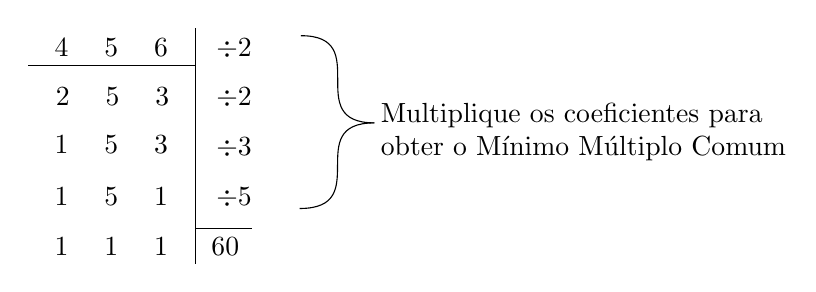
\begin{tikzpicture}[x=0.75pt,y=0.75pt,yscale=-0.6,xscale=0.6]		
		\draw    (86,100) -- (220,100) ;
		\draw    (220,70) -- (220,259) ;
		\draw    (220,231) -- (266,231) ;
		\draw    (305,76) .. controls (364,76) and (305,146) .. (364,146) ;
		\draw    (304,214.75) .. controls (364,214.75) and (305,146) .. (364,146) ;
		\draw (235,76) node [anchor=north west][inner sep=0.75pt]   [align=left] {$\div 2$};
		\draw (185,76) node [anchor=north west][inner sep=0.75pt]   [align=left] {6};
		\draw (145,76) node [anchor=north west][inner sep=0.75pt]   [align=left] {5};
		\draw (105,76) node [anchor=north west][inner sep=0.75pt]   [align=left] {4};
		\draw (235,116) node [anchor=north west][inner sep=0.75pt]   [align=left] {$\div 2$};
		\draw (235,156) node [anchor=north west][inner sep=0.75pt]   [align=left] {$\div 3$};
		\draw (235,196) node [anchor=north west][inner sep=0.75pt]   [align=left] {$\div 5$};
		\draw (231,236) node [anchor=north west][inner sep=0.75pt]   [align=left] {60};
		\draw (186,116) node [anchor=north west][inner sep=0.75pt]   [align=left] {3};
		\draw (146,116) node [anchor=north west][inner sep=0.75pt]   [align=left] {5};
		\draw (106,116) node [anchor=north west][inner sep=0.75pt]   [align=left] {2};
		\draw (185,154) node [anchor=north west][inner sep=0.75pt]   [align=left] {3};
		\draw (145,154) node [anchor=north west][inner sep=0.75pt]   [align=left] {5};
		\draw (105,154) node [anchor=north west][inner sep=0.75pt]   [align=left] {1};
		\draw (185,196) node [anchor=north west][inner sep=0.75pt]   [align=left] {1};
		\draw (145,196) node [anchor=north west][inner sep=0.75pt]   [align=left] {5};
		\draw (105,196) node [anchor=north west][inner sep=0.75pt]   [align=left] {1};
		\draw (185,236) node [anchor=north west][inner sep=0.75pt]   [align=left] {1};
		\draw (145,236) node [anchor=north west][inner sep=0.75pt]   [align=left] {1};
		\draw (105,236) node [anchor=north west][inner sep=0.75pt]   [align=left] {1};
		\draw (367,128) node [anchor=north west][inner sep=0.75pt]   [align=left] {Multiplique os coeficientes para \\obter o Mínimo Múltiplo Comum};
	\end{tikzpicture}
	\end{center}

    \noindent
	\textbf{Passo 2}: Reescrever as frações com o novo denominador, deixando o espaço do numerador para os números que serão encontrados no passo seguinte.

        \begin{texample}
        \centering
        \tcbhighmath{\frac{10}{4} + \frac{12}{5} + \frac{3}{6} =  \frac{}{60} + \frac{}{60} + \frac{}{60}}
        \end{texample}

    \noindent
	\textbf{Passo 3}: Encontre os numeradores de cada nova fração. Para isso, o seguinte cálculo deverá ser feito:

    Para encontrar o numerador da primeira fração, é necessário dividir o MMC (60) pelo denominador da primeira fração (4) e multiplicar o resultado pelo seu numerador (10). O resultado obtido por esse cálculo (150) será o numerador da primeira fração que tem denominador igual ao MMC (60). O mesmo procedimento deve ser repetido para todas as frações presentes na soma, ou seja,

        \begin{texample}
        \centering
        \tcbhighmath{\frac{10}{4} + \frac{12}{5} + \frac{3}{6} =  \frac{150}{60} + \frac{144}{60} + \frac{30}{60}}
        \end{texample}
	
	\begin{table}[htbp]
		\centering
		\caption{Passo a passo do MMC}
		\begin{tabular}{cc}
			\hline
			Memória de cálculo &  (MMC ÷ denominador) × numerador \bigstrut\\
			\hline
			Primeira fração  & (60 ÷ 4) × 10 = 150 \bigstrut[t]\\
			Segunda fração  & (60 ÷ 5) × 12 = 144 \\
			Terceira fração &  (60 ÷ 6) × 3 = 30 \\
            \hline
		\end{tabular}%
		\label{tab:addlabel}%
	\end{table}%

    \noindent
	\textbf{Passo 4}: Somar as novas frações utilizando o caso anterior (de denominadores iguais), ou seja, some os numeradores e mantenha o mesmo denominador.

        \begin{texample}
        \centering
        \tcbhighmath{\frac{10}{4} + \frac{12}{5} + \frac{3}{6} = \frac{150}{60} + \frac{144}{60} + \frac{30}{60} = \frac{150 + 144 + 30}{60} = \frac{324}{60}}
        \end{texample}
	
	\subsection{Subtração}
	Para subtrair frações deve-se ter o mesmo cuidado que tivemos na soma, ou seja, verificar se os denominadores são iguais. Se forem, deve-se repetir o denominador e subtraímos os numeradores. Se forem diferentes, faz-se os mesmos procedimentos da soma, para obter frações equivalentes de mesmo denominador. Em seguida, deve-se  efetuar a subtração. Veja o exemplo:

        \begin{texample}
        \centering
        \tcbhighmath{\frac{3}{4} - \frac{1}{5} - \frac{1}{2} = \frac{15}{20} - \frac{4}{20} - \frac{10}{20} = \frac{15 - 4 - 10}{20} = \frac{1}{20}}
        \end{texample}
	
	Efetue as seguintes operações (de soma ou subtração) com frações.
	
	\begin{tasks}
		\task $\df{3}{4} + \df{1}{1} $
		\task $ 2 - \df{3}{4} $
		\task $\df{1}{6} - \df{1}{9} + \df{1}{3} $
		\task $\df{1}{5} - \df{3}{5} + \df{2}{5} $
	\end{tasks}
	
	\subsection{Multiplicação}
	
	A multiplicação de frações é muito simples, basta multiplicar os numeradores entre si, bem como seus denominadores. Observe:

        \begin{texample}
        \centering
        \tcbhighmath{\frac{2}{3} \times \frac{5}{7} =  \frac{2 \times 5}{3 \times 7} = \frac{10}{21}}
        \tcbhighmath{\frac{6}{11} \times \frac{9}{5} =  \frac{6 \times 9}{11 \times 5} = \frac{54}{55}}
        \end{texample}
	
	\subsection{Divisão}
 
    A divisão deve ser efetuada aplicando uma regra prática e de fácil assimilação. Deve-se repetir a primeira fração e multiplicá-la pelo inverso da segunda fração (invertendo o numerador e denominador da segunda fração). Os exemplos a seguir ilustram o procedimento:

        \begin{texample}
        \centering
        \tcbhighmath{\frac{9}{2} \div \frac{7}{3} = \frac{9}{2} \times \frac{3}{7} =  \frac{9 \times 3}{2 \times 7} = \frac{27}{14}}
        \tcbhighmath{\frac{8}{3} \div \frac{5}{9} = \frac{8}{3} \times \frac{9}{5} =  \frac{8 \times 9}{3 \times 5} = \frac{72}{15}}
        \end{texample}
	
	\section{Propriedades das operações}
 
	É importante lembrar que existe uma regra de prioridade das operações. Essa regra define a ordem correta para resolver as diferentes partes de uma expressão. Usar uma regra de ordem para realizar as operações garante que uma expressão tenha solução única. Sem uma ordem definida para as operações, as expressões usadas em áreas científicas ou financeiras, por exemplo, não seriam muito úteis, e seria impossível saber se uma resposta está correta numa prova de matemática.
	
	Em qualquer operação matemática deve-se começar resolvendo os parênteses. Na verdade os sinais gráficos: 1º parênteses - \text{( )}, 2º colchetes - \text{[ ]} e 3º Chaves - \text{\{ \}}, depois os expoentes, em seguida as multiplicações e divisões e, por último, a adição e a subtração. Quando as operações são do mesmo nível (mesmo expoente), elas devem ser resolvidas da esquerda para a direita. Por exemplo, se o cálculo tiver mais de um expoente, primeiro você deve solucionar o da esquerda e continuar para a direita. A ordem padrão é a seguinte: parêntesis, expoentes, multiplicação e divisão, e finalmente, adição e subtração.
	
	Vejamos a seguinte expressão:

        \begin{texample}
        \centering
        \tcbhighmath{\dfrac{4}{2} \times 3 + (4 + 6 \times 2) + \dfrac{18}{9} - 8}
        \end{texample}
	
	\begin{enumerate}
		\item Sempre deve-se começar resolvendo as operações que estão dentro dos parênteses que servem para agrupar partes de uma expressão matemática.
            \begin{tcolorbox}[colback=white,colframe=minha_cor,coltitle=black,title=Passo 1] 
            \[
            \dfrac{4}{2} \times 3+ (4 + 6 \times 2) + \dfrac{18}{9} - 8
            \]
            \end{tcolorbox}		
		\item Dentro dos parênteses, é necessário seguir a ordem das operações como seria feito em uma expressão sem eles. No exemplo, existem duas operações: uma adição e uma multiplicação. Como a multiplicação sempre deve ser realizada primeiro, deve-se começar multiplicando $6 \times 2=12$ e, em seguida, realizar a adição $12+4=16$.
  
            \begin{tcolorbox}[colback=white,colframe=minha_cor,coltitle=black,title=Passo 2] 
            \[
            \dfrac{4}{2} \times 3+ (4 + 12) + \dfrac{18}{9} - 8
            \]
            \[
            \dfrac{4}{2} \times 3+ (16) + \dfrac{18}{9} - 8
            \]
            \end{tcolorbox}
        
		\item Agora realiza-se as operações de multiplicação ou divisão. É importante lembrar que a multiplicação não precisa ser feita necessariamente antes da divisão. Neste caso, as operações são resolvidas da esquerda para a direita. Começando pela esquerda primeiramente é necessário resolver $\frac{4}{2} = 2$
  
             \begin{tcolorbox}[colback=white,colframe=minha_cor,coltitle=black,title=Passo 3.1] 
            \[
            2 \times 3 + 16 + \frac{18}{9} - 8
            \]
            \end{tcolorbox}	
		
		a próxima operação é $2 \times 3 = 6$ 

            \begin{tcolorbox}[colback=white,colframe=minha_cor,coltitle=black,title=Passo 3.2] 
             \[
            6 + 16 + \frac{18}{9} - 8
            \]
            \end{tcolorbox}	
            		
		a última operação de divisão ou multiplicação é $\frac{18}{9} = 2$

            \begin{tcolorbox}[colback=white,colframe=minha_cor,coltitle=black,title=Passo 3.3] 
             \[
            6 + 16 + 2 - 8
            \]
            \end{tcolorbox}	
            		
		\item Não há mais nada para multiplicar ou dividir, então é possível avançar para a última 
		parte na ordem de operações: a adição e a subtração. Assim, como fizemos com as 
		multiplicações e com as divisões, adicionaremos e subtrairemos da esquerda para a 
		direita.
            \begin{tcolorbox}[colback=white,colframe=minha_cor,coltitle=black,title=Passo 4.1] 
             \[
            6 + 16 + 2 - 8
            \]
            \[
            24 - 8
            \]
            \[
            16
            \]
            \end{tcolorbox}	
		
		Em outras palavras:
            \begin{tcolorbox}[colback=white,colframe=minha_cor,coltitle=black,title=Passo 4.2] 
             \[
            \frac{4}{2} \times 3 + (4 + 6 \times 2) + \frac{18}{9} - 8 = 16
            \]
            \end{tcolorbox}				
	\end{enumerate}
	
	De forma análoga ao exemplo anterior, calcule as seguintes expressões:
	
	\begin{tasks}(2)
		\task $\df{\df{2}{5}}{3} $ \\[-0.25cm]
		\task $ \df{5}{2} + \left[2 - \left(\df{8}{3} + \df{4}{3}\right) \right] $ \\[-0.25cm]
		\task $ \left[ \df{7}{2} - \left(\df{5}{6} + \df{1}{2} \times \df{1}{3}\right) \right] $ \\[-0.25cm]
		\task $ \df{17}{3} \div \left[5 + \df{7}{5} \times \left(\df{7}{2} - \df{1}{6}\right) \right] $ \\[-0.25cm]
		\task $ [9 - (-6)] \times \left[\df{2(-3) - 4(5)}{-8(6) - 4}\right] $
	\end{tasks}
	
	\section{Exercícios}
	\begin{enumerate}
		\item Calcule as expressões a seguir e simplifique o resultado (quando possível)
		\begin{tasks}(2)
			\task $\df{3}{4} + 1 $ \\[-0.25cm]
			\task $2 - \df{2}{3} $ \\[-0.25cm]
			\task $\df{1}{3} + \df{2}{5} + \df{3}{13} $ \\[-0.25cm]
			\task $\df{7}{3} \times 2 $ \\[-0.25cm]
			\task $\df{1}{7} \div \df{2}{3} \times \df{5}{3} $ \\[-0.25cm]
			\task $\df{1}{9} \times \df{12}{7} $ \\[-0.25cm]
			\task $\df{1}{11} \div \df{4}{5} + 9 $ \\[-0.25cm]
			\task $\df{3}{7} - \df{8}{4} + 4 $ \\[-0.25cm]
			\task $\df{1}{5} - \df{2}{3} \times \df{9}{2} $ \\[-0.25cm]
			\task $\df{1}{30} \div \df{2}{15} - \df{1}{3} $
		\end{tasks}
		
		\item Calcule as expressões a seguir e simplifique o resultado (quando possível)
		\begin{tasks}(2)
			\task $\df{\,\df{2}{5}\,}{3} $ \\[-0.25cm]
			\task $\df{5}{6} - \left(\df{2+3}{7}\right) $ \\[-0.25cm]
			\task $\left(\df{1}{4} + \df{1}{2}\right) \div \left(\df{3}{2} + 3\right) $ \\[-0.25cm]
			\task $9 - 3 \div \df{1}{3} + 1 $\\[-0.25cm]
			\task $\df{5}{2} + \left[2 - \left(\df{8}{3} + \df{4}{3}\right)\right] $ \\[-0.25cm]
			\task $\df{\df{6}{9} \div \df{1}{3} + 6}{\df{4}{3} \div \df{1}{6} + \df{6}{5} \times \df{2}{30}} $ \\[-0.25cm]
			\task $\df{\df{4}{3} \times \df{1}{2} - 2}{\df{2}{3} \div \df{1}{3} + \df{6}{5} \times \df{2}{3}} $ \\[-0.25cm]
			\task $3 \times \df{9}{4} - {\left[\left(\df{2}{3}\right)^2 + 2\right] \div \sqrt{\df{4}{9}}} $ \\[-0.25cm]
			\task $\left[ \left(\df{2}{3} \div \left(\df{1}{10}\right)^2 - 10^3\right)\right] $ \\[-0.25cm]
			\task $\df{\df{4}{3} \times \df{1}{8}}{\df{3}{7} + \df{16}{9} \times \df{7}{2}} $
		\end{tasks}
		
		\item A expressão  $\df{1 + \df{1}{1 -\df{1}{5}}}{-1 + \df{3}{1 +\df{1}{5}}}$ é equivalente a:
		\begin{enumerate}
			\item $\df{2}{3}$
			\item $\df{3}{2}$
			\item $\df{1}{3}$
			\item $\df{1}{4}$
			\item $0$
		\end{enumerate}
		
		\item O valor da expressão  $ \left[9 \times \left(\df{\df{2}{3} + \df{3}{2}- \df{5}{6} - \df{2}{12}}{\df{8}{5} \times \df{3}{8} \div 2 + 1 + \df{1}{2}}\right) + \df{1}{3} \times \df{1}{2}\right]$ é:
		\begin{enumerate}
			\item $\df{2}{3}$
			\item $\df{3}{2}$
			\item $\df{1}{3}$
			\item $\df{1}{4}$
			\item $0$
		\end{enumerate}
		
		\item A expressão  $\df{5 + \left(\df{2}{4}\right)^2}{1 + \df{8}{8 + \sqrt{\df{9}{100}}}}$ equivale a:
		\begin{enumerate}
			\item $\df{11}{4}$
			\item $\df{230}{82}$
			\item $\df{77}{29}$
			\item $\df{2770}{1012}$
			\item $\df{13}{5}$
		\end{enumerate}
	\end{enumerate}
	
	\newpage
	
	\section{Respostas dos exercícios}
 
	\begin{enumerate}
		\item 
		\begin{tasks}(3)
			\task $\df{7}{4}$ \\[-0.25cm]
			\task $\df{4}{3}$ \\[-0.25cm]
			\task $\df{188}{195}$ \\[-0.25cm]
			\task $\df{14}{3} $ \\[-0.25cm]
			\task $\df{5}{14}$ \\[-0.25cm]
			\task $\df{4}{21}$ \\[-0.25cm]
			\task $\df{401}{44}$ \\[-0.25cm]
			\task $\df{17}{7}$ \\[-0.25cm]
			\task $-\df{14}{5}$ \\[-0.25cm]
			\task $-\df{1}{12}$ \\[-0.25cm]
		\end{tasks}
  
		\item 
		\begin{tasks}(3)
			\task $\df{2}{15}$ \\[-0.25cm]
			\task $\df{5}{42}$ \\[-0.25cm]
			\task $\df{1}{6}$ \\[-0.25cm]
			\task $1$ \\[-0.25cm]
			\task $\df{1}{2}$ \\[-0.25cm]
			\task $\df{216}{181}$ \\[-0.25cm]
			\task $-\df{10}{21}$ \\[-0.25cm]
			\task $\df{37}{12}$ \\[-0.25cm]
			\task $0$ \\[-0.25cm]
			\task $-\df{735}{3352}$
		\end{tasks}
		\item Alternativa (b) $ = \df{3}{2}$
		\item Alternativa (d) $ = 1$
		\item Alternativa (a) $ = \df{11}{4}$
	\end{enumerate}
	
	\newpage
	
	\section*{Anexo A}
 
	Para saber mais sobre frações, separamos alguns vídeos interessantes que servirão de base para o estudo.\\

 
	\begin{enumerate}
		\item O que é fração? 
		Ideias das Frações e o que são frações \\[-0.5cm]
  
		{\color{red} \;\Large \faIcon{youtube}} \;Link: \url{https://youtu.be/55sqKNqgK8s}
		\item Tipos de frações
		\begin{enumerate}
			\item Própria, Aparente, Mista e Imprópria \\[-0.5cm]
   
		      {\color{red} \;\Large \faIcon{youtube}} Link: \url{https://youtu.be/C6D62Or8HcA}
			\item O que são Frações Equivalentes e Frações Irredutíveis \\[-0.5cm]
   
		      {\color{red} \;\Large \faIcon{youtube}} Link: \url{https://youtu.be/AMjr5IgaAS4}
		\end{enumerate}
		\item Operações com frações
		\begin{enumerate}
			\item MMC | Mínimo Múltiplo Comum \\[-0.5cm]
   
			{\color{red} \;\Large \faIcon{youtube}} Link: \url{https://youtu.be/02NUuEKseEg}
			\item Adição e Subtração de Frações | Denominadores iguais e diferentes \\[-0.5cm]
   
			{\color{red} \;\Large \faIcon{youtube}} Link: \url{https://youtu.be/HmtEOJ-CXds} 
			\item Como fazer Multiplicação de Frações | Significado Geométrico \\[-0.5cm]
   
			{\color{red} \;\Large \faIcon{youtube}} Link: \url{https://youtu.be/oc-oHcItwJE}
			\item Divisão de Frações | Interpretação Geométrica e Aritmética \\[-0.5cm]
   
			{\color{red} \;\Large \faIcon{youtube}} Link: \url{https://youtu.be/bbw9kwj3g7U}
		\end{enumerate}
	\end{enumerate}